%
% chapter.tex -- Skalarprodukt
%
% (c) 2021 Prof Dr Andreas Müller, Hochschule Rapperswil
%
% !TeX spellcheck = de_CH
\chapter{Diskrete harmonische Analysis
\label{buch:chapter:diskret}}
\kopflinks{Skalarprodukte}

%
% 1-endlich.tex
%
% (c) 2023 Prof Dr Andreas Müller, OST Ostschweizer Fachhochschule
%
\section{Endliche Gruppen
\label{buch:diskret:section:endlich}}
\kopfrechts{Endliche Gruppen}
Diskrete Fourier-Analysis handelt von der Fourier-Theorie auf
endlichen abelschen Gruppen.
Dieser Abschnitt treibt die Theorie der endlich erzeugten Gruppen
weit genug, damit wir alle endlichen abelschen Gruppen beschreiben
können.

%
% Endlich erzeugt Gruppen
%
\subsection{Endlich erzeugte Gruppen
\label{buch:diskret:endlich:subsetion:endlicherzeugt}}
Endliche Gruppen enthalten nur endlich viele Elemente, die Gruppenoperationen
können daher leicht durch eine Multiplikations oder Invertierungstabelle
vollständig beschrieben werden.
In diesem Abschnitt soll gezeigt werden, dass sogar noch viel weniger
nötig ist, weil solche Gruppen aus einer kleineren Menge von Elementen
Erzeugt werden können.

\begin{definition}
Sei $F\subset G$ eine Teilmenge einer Gruppe $G$.
Dann heisst die kleinste Untergruppe $\langle F\rangle$ von $G$,
der $F$ enthält, die von $F$ erzeugte Gruppe.
\end{definition}

\begin{beispiel}
Sei $\mathbb{R}$ die additive Gruppe der reellen Zahlen und
\[
F
=
\biggl\{\frac{1}{p^k}
\;
\bigg|
\;
\text{$p$ ist Primzahl, $k\in\mathbb{N}$}\biggr\}
\]
eine Teilmenge.
Die erzeugte Untergruppe enthält sicher alle Brüche der Form
\[
\frac{a}{p^k},\quad a\in\mathbb{Z},k\in\mathbb{N},\text{$p$ prim}.
\]
Da aber auch Summen von Brüchen der Form
\[
\frac{a}{p^k} + \frac{b}{q^l}
=
\frac{aq^l+bp^k}{p^kq^l}
\]
enthalten, die erzeugte Gruppe muss daher auch alle Brüche mit
Nennern erhalten, die Produkte von beliebigen Primzahlpotenzen sind.
Da jeder Nenner als Primzahlprodukt geschrieben werden kann, folgt,
dass die von $F$ erzeugte Gruppe alle rationalen Zahlen enthalten
muss.
Da aber in $F$ nur rationale Zahlen vorhanden sind, folgt
$\langle F\rangle = \mathbb{Q}$.
\end{beispiel}

\begin{satz}
Die erzeugte Gruppe der Teilmenge $F$ der Gruppe $G$ ist
\[
\langle F\rangle
=
\bigcap_{F\subset H\subset G \atop\text{$H$ Gruppe}} H
\]
\end{satz}

\begin{definition}
Eine Gruppe $G$ heisst {\em endlich erzeugt}, wenn es eine endliche Menge
$F\subset G$ gibt derart, dass $G=\langle F\rangle$.
\end{definition}

\begin{beispiel}
Die Menge $F=\{n\}\subset\mathbb{Z}$ erzeugt die additive Untergruppe
\[
\langle F \rangle
=
\{\dots,-3n,-2n,-n,0,n,2n,3n,\dots\}
=
n\mathbb{Z}.
\]
Für eine endliche Teilmenge $F=\{n_1,\dots,n_k\}\subset\mathbb{Z}$
besteht die erzeugte additive Untergruppe
\[
\langle F\rangle
=
\operatorname{ggT}(n_1,\dots,n_k)\mathbb{Z}
\]
aus den Vielfachen des grössten gemeinsamen Teilers der Zahlen
$n_1,\dots,n_k$.
\end{beispiel}

\begin{beispiel}
Sei $\alpha\in \mathbb{R}$, dann besteht die von $e^{i\alpha}$ erzeugte
multiplikative Untergruppe von $\mathbb{C}^*$ aus den Elementen
\[
\langle e^{i\alpha}\rangle
=
\{ e^{in\alpha}\mid n\in\mathbb{Z}\}.
\]
Sie ist genau dann eine endliche Gruppe, wenn es eine Zahl $l\in\mathbb{Z}$
mit $e^{il\alpha}=1$.
Dies ist gleichbedeutend damit, dass $l\alpha$ ein Vielfaches von $2\pi$
ist, also $l\alpha = 2\pi k$ mit $k\in\mathbb{Z}$.
Somit ist 
\[
\alpha = 2\pi \frac{k}{l},
\]
ein rationales Vielfaches von $\pi$.
Ohne Beschränkung der Allgemeinheit darf man annehmen, dass $k$ und $n$
teilerfremd sind, dass also der Bruch $k/n$ gekürzt ist.
Die Zahlen $e^{in\alpha}=e^{2\pi i n (k/l)}$ sind gleich, wenn 
sich die Exponenten nur um ein Vielfaches von $2\pi i$ unterscheiden,
wenn also $nk$ den gleichen Rest module $l$ haben.
Da $k$ und $l$ teilerfremd sind, sind alle Reste module $l$ möglich.
Die erzeugte endliche Untergruppe ist also
\[
\langle e^{i\alpha}\rangle
=
\{ e^{2\pi i nk/l}\mid n\in \mathbb{Z} \}
=
\{ e^{2pi i n/l} \mid n=0,\dots,l-1 \}
=
C_l
\]
die zyklische Untergruppe der Ordnung $l$.

Falls $\alpha$ kein rationales Vielfaches von $\pi$ ist, ist die
erzeugte Gruppe eine unendliche Untergruppe von komplexen Zahlen vom
Betrag $1$.
Eine solche Gruppe ist eine Menge, die in
$S^1=U(1)=\{z\in\mathbb{C}^*\mid |z|=1\}$
dicht liegt.
\end{beispiel}

%
% Produkte
%
\subsection{Produkte
\label{buch:diskret:endlich:subsection:produkte}}
Die Ordnung einer abelschen Gruppe charakterisiert die Struktur einer
Gruppe noch nicht eindeutig.
In diesem Abschnitt soll gezeigt werden, wie sich aus endlichen
Gruppen neue zusammensetzen lassen.

Seien $G$ und $H$ endliche Gruppen.
Dann lässt sich eine neue Gruppe konstruieren, die auch die
{\em Produktgruppe} heisst.
Sie besteht besteht aus den Paaren von Gruppenelementen
\[
G\times H
=
\{ (g,h) \mid g\in G\text{ und } h\in H\}.
\]
Die Verknüpfung ist
\begin{align*}
(g_1,h_1)(g_2,h_2)
&=
(g_1g_2,h_1h_2)
\intertext{mit dem neutralen Element}
e_{G\times H}
&=
(e_G,e_H)
\intertext{wobei $e_G$ und $e_H$ die neutralen Elemente von $G$ bzw.~$H$
sind.
Das inverse Element ist dann}
(g,h)^{-1}
&=
(g^{-1},h^{-1}).
\end{align*}

Sind die Gruppen $G_1$ und $G_2$ endlich erzeugt mit den Erzeugendensystemen
$F_1$ bzw.~$F_2$, dann ist die Menge
\[
F
=
F_1\times \{e_2\}
\cup
\{e_1\} \times F_2
=
\{ (f,e_2) \in G_1\times G_2 \mid f\in G_1 \}
\cup
\{ (e_1, f) \in G_1\times G_2 \mid f\in G_2 \},
\]
wobei $e_k$ das neutrale Element der Gruppe $G_k$, $k=1,2$ ist.
Die Menge $F$ ist endlich, denn $|F| = |F_1| + |F_2|$.
Damit ist gezeigt, dass das Produkt endlich erzeugter Gruppen 
wieder endlich erzeugt ist.

\begin{satz}
Sind $G_1$ und $G_2$ endlich erzeugte Gruppen, dann ist auch
$G_1\times G_2$ endlich erzeugt.
\end{satz}

Die Verknüpfung abelscher Gruppen wird oft additiv geschrieben.
In diesem Fall wird die Produktgruppe auch als {\em direkte Summe}
\[
G\times H
=
G\oplus H
\]
geschrieben mit der Verknüpfung
\begin{align*}
(g_1,h_1) + (g_2,h_2)
&=
(g_1+g_2,h_1+h_2)
\\
-(g,g)&=(-g,h)
\intertext{und dem neutralen Element}
0&= (0,0).
\end{align*}
Die direkte Summe ist auch wieder eine abelsche Gruppe.

\begin{figure}
\centering
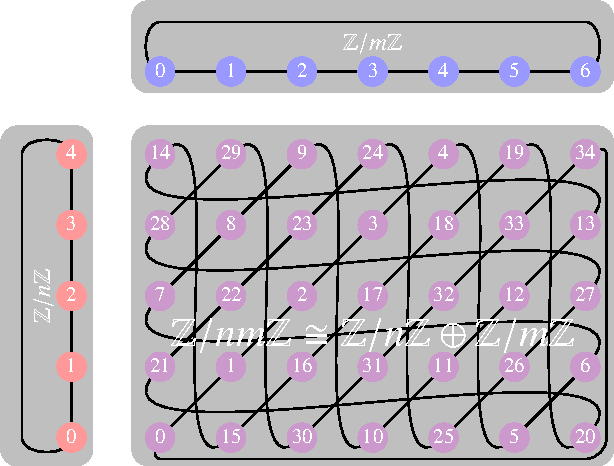
\includegraphics{chapters/060-diskret/images/faktoren.pdf}
\caption{Das Produkt der Gruppen $\mathbb{Z}/n\mathbb{Z}$ und
$\mathbb{Z}/m\mathbb{Z}$ ist für teilerfremde Zahlen $n$ und $m$
isomorph zu $\mathbb{Z}/nm\mathbb{Z}$.
\label{buch:diskret:endlich:fig:produkt}}
\end{figure}

\begin{satz}
\label{buch:diskret:endlich:satz:teilerfremd}
Sind $n$ und $m$ teilerfremd, dann ist
$
\mathbb{Z}/nm\mathbb{Z}
\equiv
\mathbb{Z}/n\mathbb{Z} \oplus \mathbb{Z}/m\mathbb{Z}
$.
\end{satz}

\begin{proof}[Beweis]
Das Element $(1,1)\in \mathbb{Z}/n\mathbb{Z}\oplus\mathbb{Z}/m\mathbb{Z}$
hat die Eigenschaft $nm(1,1)=(0,0)$.
Ausserdem gibt es keine Zah $k<nm$, für die $k(1,1)=(0,0)$ ist, denn
dazu müsste $k$ ein Teiler von $n$ und $m$ sein, was nach Voraussetzung
verboten ist.
\end{proof}

Der in Abbildung~\ref{buch:diskret:endlich:fig:produkt} illustrierte
Satz zeigt, dass sich eine endlich erzeugte abelsche Gruppe immer
Summanden der Form $\mathbb{Z}/p^k\mathbb{Z}$ für Primzahlen $p$
zerlegen lässt.
Es bleibt dann nur noch zu untersuchen, ob die Gruppen für verschiedene
$k$ verschieden sind oder sich weiter zerlegen lassen.
Darauf gibt der folgende Satz eine Antwort.

\begin{satz}
\label{buch:diskret:endlich:satz:ppotenz}
Die Gruppen $\mathbb{Z}/p^k\mathbb{Z}$ und $\mathbb{Z}/p^l\mathbb{Z}$
sind nicht isomorph, wenn $k\ne l$.
\end{satz}

\begin{proof}[Beweis]
Sei $k>l$, dann ist  auch $p^k>p^l$.
Für jedes Element $x \in \mathbb{Z}/p^l\mathbb{Z}$ gilt, 
$p^lx=0$.
Das Element $1\in \mathbb{Z}/p^k\mathbb{Z}$ hat diese Eigenschaft
nicht, also können die beiden Gruppen nicht isomorph sein.
\end{proof}

%
% Struktursatz
%
\subsection{Der Struktursatz
\label{buch:diskret:endlich:subsection:}}
Ausgehend von den beiden Sätzen~\ref{buch:diskret:endlich:satz:teilerfremd}
und
\ref{buch:diskret:endlich:satz:ppotenz}
ist jetzt der folgende Struktursatz für endlich erzeugte abelsche
Gruppen plausibel.

\begin{satz}
\label{buch:diskret:endlich:struktursatz}
Ist $G$ eine endliche erzeugte abelsche Gruppe, dann gibt es eine
Zahl $d\in\mathbb{N}$ und eindeutig bestimmte Primzahlpotenzen $d_i$
derart, dass
\[
G
\cong
\mathbb{Z}^d
\oplus
\bigoplus_{i=1}^n
\mathbb{Z}/d_i\mathbb{Z}.
\]
Die Ordnung der Gruppe $G$ ist $|G|=\prod_{i=1}^n d_i$.
\end{satz}

%
% Die duale Gruppe
%
\subsection{Die duale Gruppe
\label{buch:diskret:endlich:subsection:dual}}
Für die Fourier-Theorie für Funktionen mit einer endlich erzeugten
Gruppe $G$ muss die duale Gruppe ermittelt werden.
Aus dem Struktursatz~\ref{buch:diskret:endlich:struktursatz}
für endlich erzeugte Gruppen folgt, dass ein Homomorphismus
$G\to\mathbb{C}$ durch die Werte auf den erzeugenden Elementen
jedes einzelnen Summanden eindeutig bestimmt ist.
Daher gilt der folgende Satz:

\begin{satz}
Ist $G$ eine endlich erzeugte Gruppe, dann ist
$\hat{G}\cong G$.
\end{satz}

\begin{proof}[Beweis]
Sei
\[
G
=
\bigoplus_{i=1}^k \mathbb{Z}/d_i\mathbb{Z}
\]
die Zerlegung von $G$ gemäss dem Struktursatz
\ref{buch:diskret:endlich:struktursatz}.
Es ist jetzt nur noch zu zeigen, dass die duale Gruppe einer direkten
Summe die direkte Summe der dualen Gruppen ist, dass also
$(G_1\oplus G_2)\hat{\phantom{\imath}} \cong \hat{G}_1\oplus \hat{G}_2$.
\end{proof}

Die duale Gruppe der Gruppe $G$ besteht aus den Homomorphismen
$G\to\mathbb{C}^*$.
Ein Homomorphismus $\varphi\colon G\to H$ führt daher auf den
Homomorphisums
\[
\hat{\varphi}
\colon
\hat{H}\to\hat{G}
:
f\mapsto f\circ \varphi
\]
der dualen Gruppen.
Das Produkt der Gruppen $G_1$ und $G_2$ kann durch die Projektionsabbildungen
\[
\renewcommand{\arraycolsep}{2pt}
\begin{array}{rl}
\pi_1 \colon G_1 \oplus G_2 \to G_1 : (x,y) \mapsto {}&x
\\
\pi_2 \colon G_1 \oplus G_2 \to G_2 : (x,y) \mapsto {}&y
\end{array}
\]
und die Einbettungen
\[
\renewcommand{\arraycolsep}{2pt}
\begin{array}{rcl}
i_1 \colon G_1 \to G_1\oplus G_2 : &x&\mapsto (x,0) \\
i_2 \colon G_2 \to G_1\oplus G_2 : &y&\mapsto (0,y) 
\end{array}
\]
charakterisiert werden.
Die dualen Homomorphismen
$\hat{\pi}_k\colon\hat{G}_k\to (G_1\oplus G_2)\hat{\phantom{\imath}}$
und
$\hat{\imath}_k\colon (G_1\oplus G_2)\hat{\phantom{\imath}}\to\hat{G}_k$
können verwendet werden, um $\hat{G}_1\oplus\hat{G}_2$ und
$(G_1\oplus G_2)\hat{\phantom{\imath}}$ miteinander zu verbinden.

Ist $f\colon G_1\oplus G_2\to\mathbb{C}^*$ ein Homomorphismus, dann 
sind $\hat{\imath}_k(f)$ für $k=1,2$ Homomorphismen $G_k\to\mathbb{C}^*$
mit dem Wert
\[
\hat{\imath}_k(f)(g)
=
f(i_k(g))
=
\begin{cases}
f(g,0)&\qquad k=1\\
f(0,g)&\qquad k=2.
\end{cases}
\]
Umgekehrt bildet $\hat{\pi}_k$ für $k=1,2$ einen Homomorphismus
$f_k\colon \hat{G}_k\to\mathbb{C}^*$ auf den
Homomorphismus
\[
\hat{\pi}_k(f_k)
\colon
G_1\oplus G_2
\to
\mathbb{C}^*
:
(g_1,g_2)
\mapsto
h(\pi_k(g_1,g_2)) = h(g_k)
\]
ab.

Die Homomorphismen $\pi_k$ und $i_k$ erfüllen
$\pi_k \circ i_k=\operatorname{id}_{G_k}$.
Für die dualen Homomorphismen muss daher
$\hat{\imath}_k\circ\hat{\pi}_k=\operatorname{id}_{\hat{G}_k}$
gelten.
Daraus können wir jetzt die Homomorphismen 
\[
\renewcommand{\arraycolsep}{2pt}
\begin{array}{rcrclcrclcrcl}
\hat{\pi}_1 \oplus \hat{\pi}_2
&\colon&
\hat{G}_1\oplus\hat{G}_2\phantom{)\hat{\imath}}
&\to&
(G_1\oplus G_2)\hat{\phantom{\imath}}
&:&
(f_1,f_2)
&\mapsto&
\hat{\pi}_1(f_1) + \hat{\pi}_2(f_2)
&:&
(g_1,g_2)
&\mapsto&
f_1(g_1)+f_2(g_2)
\\
(\hat{\imath}_1 , \hat{\imath}_2)
&\colon&
(G_1\oplus G_2)\hat{\phantom{\imath}}
&\to&
\phantom{(}
\hat{G}_1\oplus\hat{G}_2
&:&
f
&\mapsto&
(\hat{\imath}_1(f), \hat{\imath}_2(f))
&&
&&
\end{array}
\]
konstruieren.
Wir berechnen die Zusammensetzungen in beiden möglichen Reihenfolgen.
Die Zusammensetzung
$(\hat{\pi}_1\oplus\hat{\pi}_2)\circ(\hat{\imath}_1,\hat{\imath}_2)$
bildet einen Homomorphismus $f\colon G_1\oplus G_2\to\mathbb{C}^*$
auf den Homomorphismus ab, der auf $(g_1,g_2)\in G_1\oplus G_2$ den
Wert
\[
((\hat{\pi}_1\oplus\hat{\pi}_2)\circ(\hat{\imath}_1,\hat{\imath}_2)(f))(g_1,g_2)
=
f(g_1,0) + f(0,g_2)
=
f(g_1,g_2)
\]
annimmt, also mit $f$ identisch ist.
Dies beweist, dass
$
(\hat{\pi}_1\oplus\hat{\pi}_2)\circ(\hat{\imath}_1,\hat{\imath}_2)
=
\operatorname{id}_{(G_1\oplus G_2)\hat{\phantom{\imath}}}
$.
Aber auch die umgekehrte Zusammensetzung lässt sich direkt berechnen.
Sie bildet das Paar $(f_1,f_2)\in \hat{G}_1\oplus \hat{G}_2$ von
Homomorphismen $f_k\colon G_k\to\mathbb{C}^*$ auf das Paar
\[
(f_1',f_2')
=
(\hat{\imath}_1,\hat{\imath}_2)
\circ
(\hat{\pi}_1\oplus\hat{\pi}_2)
(f_1,f_2)
\]
ab.
Seien $g_k\in G_k$ Elemente der Gruppen $G_k$, $k=1,2$.
Wir berechnen die Werte $f_k'(g_k)$:
\begin{align*}
f_1'(g_1)
&=
(
f_1\circ\pi_1\circ i_1
\oplus
f_2\circ\pi_2\circ i_1
)(g_1)
=
f_1(\pi_1(g_1,0))
+
f_2(\underbrace{\pi_2(g_1,0)}_{\displaystyle=0})
)=
f_1(g_1) \qquad\text{und}
\\
f_2'(g_2)
&=
(
f_1\circ\pi_1\circ i_2
\oplus
f_2\circ\pi_2\circ i_2
)(g_2)
=
f_1(\underbrace{\pi_1(0,g_2)}_{\displaystyle=0})
+
f_2(\pi_2(0,g_2))
)=
f_2(g_2),
\end{align*}
die Homomorphismen $f_k'$ stimmen also mit $f_k$ überein und damit ist
\[
(\hat{\imath}_1,\hat{\imath}_2)\circ (\hat{\pi}_1\oplus\hat{\pi}_2)
=
\operatorname{id}_{\hat{G}_1\oplus\hat{G}_2}.
\]
die beiden Homomorphismen $(\hat{\imath}_1,\hat{\imath}_2)$ und
$\hat{\pi}_1\oplus\hat{\pi}_2$ sind also zueinander invers.
Damit ist der folgende Satz beweisen.

\begin{satz}
Sind $G_1$ und $G_2$ abelsche Gruppen, dann sind die Abbildungen
\begin{align*}
\hat{\pi}_1\oplus\hat{\pi}_2
&\colon
(G_1\oplus G_2)\hat{\phantom{\imath}}
\to
\hat{G}_1 \oplus \hat{G}_2
\intertext{und}
(\hat{\imath}_1,\hat{\imath}_2)
&\colon
\hat{G}_1\oplus \hat{G}_2
\to
(G_1\oplus G_2)\hat{\phantom{\imath}}
\end{align*}
zueinander inverse Isomorphismen und
$\hat{G}_1\oplus\hat{G}_2\cong(G_1\oplus G_2)\hat{\phantom{\imath}}$.
\end{satz}





%
% 2-aufloesung.tex
%
% (c) 2022 Prof Dr Andreas Müller, OST Ostschweizer Fachhochschule
%
\section{Auflösung einer Gruppe
\label{buch:diskret:section:aufloesung}}
\kopfrechts{Auflösung einer Gruppe}

%
% 3-schnell.tex
%
% (c) 2022 Prof Dr Andreas Müller, OST Ostschweizer Fachhochschule
%
\section{Schnelle Algorithmen
\label{buch:diskret:section:schnell}}
\kopfrechts{Schnelle Algorithmen}


%
% 4-koerper.tex
%
% (c) 2022 Prof Dr Andreas Müller, OST Ostschweizer Fachhochschule
%
\section{Endliche Körper
\label{buch:diskret:section:koerper}}
\kopfrechts{Endliche Körper}


%\section*{Übungsaufgaben}
%\rhead{Übungsaufgaben}
%\aufgabetoplevel{chapters/010-potenzen/uebungsaufgaben}
%\begin{uebungsaufgaben}
%\uebungsaufgabe{101}
%\uebungsaufgabe{102}
%\uebungsaufgabe{103}
%\uebungsaufgabe{104}
%\end{uebungsaufgaben}

